\chapter{Upload Process}\label{chap:process}

This chapter explains the whole process of uploading posts on the website, from filling out the Google form (Section \ref{sec:googleform}) linked to a database on Google Sheet (Section \ref{sec:googlesheet}), to running the Python code (Section \ref{sec:Python}) that formats the data into text that can be copy-pasted onto the website (Section \ref{sec:upload}). A flowchart summarizing the process is available below (Fig \ref{fig:flowchart}).

\begin{landscape}
    %\documentclass{standalone}
%\usepackage{tikz}
%\def\checkmark{\tikz\fill[scale=0.4](0,.35) -- (.25,0) -- (1,.7) -- (.25,.15) -- cycle;} 
%\usetikzlibrary{arrows,shapes,positioning,shadows,trees}
%\usetikzlibrary{decorations.markings}

%\begin{document}

\tikzstyle{startstop} = [rectangle, rounded corners, 
minimum width=3cm, 
minimum height=1cm,
text centered, 
draw=black, 
fill=red!30]

\tikzstyle{io} = [trapezium, 
trapezium stretches=true, % A later addition
trapezium left angle=70, 
trapezium right angle=110, 
text width=3cm, 
minimum width=3cm, 
minimum height=1cm, text centered, 
draw=black, fill=blue!30]

\tikzstyle{process} = [rectangle, 
minimum width=3cm, 
minimum height=1cm, 
text centered, 
text width=3cm, 
draw=black, 
fill=orange!30]

\tikzstyle{decision} = [diamond, 
minimum width=.5cm, 
aspect=2,
minimum height=.5cm,  
text width=2cm, 
text centered, 
draw=black, 
fill=green!30]
\tikzstyle{arrow} = [thick,->,>=stealth]

\begin{figure}[h!]
    \centering
    \begin{tikzpicture}[node distance=2cm]
        \vspace{1cm}
        
        \node (inform) [io] {Input (User/IPPOG)};
        \node (form) [startstop, below of=inform, yshift=-.5cm] {Google form};
        
        \node (online) [process, below of=form, yshift=-.5cm] {Google sheet database};
        \node (inonline) [io, below of=online, yshift=-.5cm] {Correction (IPPOG)};
        
        \node (decision) [decision, right of=online, xshift=2.5cm] {Choice};
        
        \node (inlocal) [io, above of=decision, yshift=.5cm] {Download CSV File (IPPOG)};
        \node (local) [process, right of=inlocal, xshift=2.5cm] {Local CSV file database};
        
        \node (inpylocal) [io, right of=local, xshift=2.5cm] {run\_local.py (IPPOG)};
        \node (pylocal) [process, right of=inpylocal, xshift=2.5cm] {Python local code};
        \node (inpyonline) [io, below of=inpylocal, yshift=-.5cm] {run\_online.py (IPPOG)};
        \node (pyonline) [process, right of=inpyonline, xshift=2.5cm] {Python online code};
        
        \node (md) [process, below of=pyonline, xshift=2.5cm, yshift=-.5cm] {Markdown files};
        
        \node (inmd) [io, below of=md, yshift=-.5cm, xshift=-2.5cm] {Copy/Past (IPPOG)};
        
        \node (web) [startstop, left of=inmd, xshift=-3cm] {Upload to Website};

        \begin{scope}[very thick,decoration={
            markings,
            mark=at position 0.7 with {\arrow{latex}}}
            ] 
            \draw [postaction={decorate}] (0,2) -- (inform);
            \draw [postaction={decorate}] (form) -- node [left] {Auto} (online);
            \draw [postaction={decorate}] (inform) -- (form);
            \draw [postaction={decorate}] (inonline) -- node [right] {Add tags and change status to "OK"}  (online);
            \draw [postaction={decorate}] (online) -- (decision);
            \draw [postaction={decorate}] (decision) -- node [above] {"online" mode} (inpyonline);
            \draw [postaction={decorate}] (decision) -- node [right] {"local" mode} (inlocal);
            \draw [postaction={decorate}] (inlocal) -- (local);
            \draw [postaction={decorate}] (local) -- (inpylocal);
            \draw [postaction={decorate}] (inpylocal) -- (pylocal);
            \draw [postaction={decorate}] (inpyonline) -- (pyonline);
            \draw [postaction={decorate}] (pylocal) -| +(2.5,-2.5);
            %\draw [postaction={decorate}] (pyonline) -+ (21.5,0);
            \draw [postaction={decorate}] (pyonline) -| (md);
            \draw [postaction={decorate}] (pyonline) -- +(2.5,0);
            %\draw [postaction={decorate}] (pylocal) -| (md);
            \draw [postaction={decorate}] (md) |- (inmd);
            \draw [postaction={decorate}] (inmd) -- (web);
            \draw [dotted,postaction={decorate}] (md) -- node [below] {Possible to do correction but need to be recompiled} (inonline);
            \draw [dotted,postaction={decorate}] (web) -- node [below] {Change status to "Online"} (-2.5,-10);
            \draw [dotted,postaction={decorate}] (-2.5,-10) |- (online);
        \end{scope}
    \end{tikzpicture}
    \caption{Flowchart of the upload process}
    \label{fig:flowchart}
\end{figure}


%\end{document}%\label{fig:flowchart}
\end{landscape}

\section{Submitting projects through the Google Form}\label{sec:googleform}

To facilitate the filling of the database, it was decided to use the option of linking a Google form to a Google Sheet document. It allows to guide the user through the form (Fig. \ref{fig:gform}), and to automatically fill the database on Google Sheet.

All fields of the form are detailed in Table \ref{tab:form_description}, with a description and whether the field is mandatory or not. It is important that the user follows the explicit format, in the case of the authors: "Author1,Afficiation1\textbackslash n" and write the full URLs including "http". Otherwise, the Python code formatting the database will not understand and will not recognize it. 

\begin{figure}[h!]
    \centering
    \begin{subfigure}[c]{.6\textwidth}
        \centering
        
\includegraphics[width=\linewidth]{Image/Process/gform.png}
    \end{subfigure}
    \bigskip
    \begin{subfigure}[c]{.6\textwidth}
        \centering
        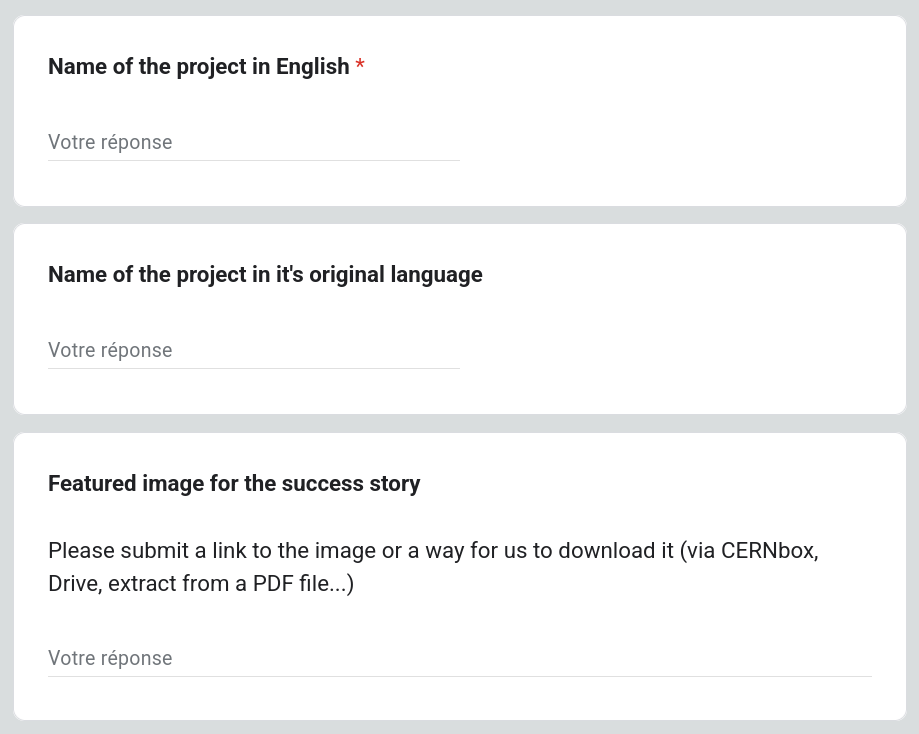
\includegraphics[width=\linewidth]{Image/Process/gform2.png}
    \end{subfigure}
    \caption{Google form interface}
    \label{fig:gform}
\end{figure}

\begin{landscape}
    \begin{table}[]
        \begin{tabularx}{\linewidth}{|lc|X|}
            \hline
            \multicolumn{1}{|l|}{\textbf{Name}} & \textbf{\begin{tabular}[c]{@{}l@{}}Mandatory\\\end{tabular}} & \textbf{Description} \\ \hline
            \multicolumn{2}{|c|}{\textbf{Main}} &  \\ \hline
            \rowcolor[HTML]{EFEFEF}
            \multicolumn{1}{|l|}{Name of the project in English} & \checkmark &  \\ \hline
            \multicolumn{1}{|l|}{Name of the project in its original language} & &  \\ \hline
            \multicolumn{1}{|l|}{Featured image for the success story} & & Link to the image or a way for us to download it \\ \hline
            \multicolumn{1}{|l|}{Credit of the featured image} & &  \\ \hline
            \rowcolor[HTML]{EFEFEF}
            \multicolumn{1}{|l|}{Abstract of the Project} & \checkmark & Abstract should be about 500 characters \\ \hline
            \multicolumn{2}{|c|}{\textbf{Contact}} &  \\ \hline
            \rowcolor[HTML]{EFEFEF}
            \multicolumn{1}{|l|}{Authors of the project and affiliations} & \checkmark & \begin{tabular}[c]{@{}l@{}}The input should take the form: \\ Author1,Afficiation1\\ Author2,Affiliation2\\ ...\\ With one author per line with no space, otherwise it will not be\\recognized by the python code\end{tabular} \\ \hline
            \rowcolor[HTML]{EFEFEF}
            \multicolumn{1}{|l|}{Public contact} & \checkmark & If an email is given, the @ sign should be replaced by "{[} at {]}" on the website (this is done automatically by the python program) \\ \hline
            \multicolumn{1}{|l|}{Private contact for the core team} & & This should not appear on the website, only in the private database \\ \hline
            \rowcolor[HTML]{EFEFEF}
            \multicolumn{1}{|l|}{Status of the project} & \checkmark & multiple choice \\ \hline
            \multicolumn{2}{|c|}{\textbf{Presented conference / meeting}} &  \\ \hline
            \multicolumn{1}{|l|}{Name of the conference / meeting} & &  \\ \hline
            \multicolumn{1}{|l|}{Year of the conference / meeting} & &  \\ \hline
            \multicolumn{1}{|l|}{URL to the presentation slides / publication} & &  \\ \hline
            \multicolumn{2}{|c|}{\textbf{Related resources}} &  \\ \hline
            \multicolumn{1}{|l|}{Other project resources} & & \begin{tabular}[c]{@{}l@{}}The input should take the form: \\ ResourceName1:URL1\\ ResourceName2:URL2\\ ...\\ With one resource per line and URL beginning by http, otherwise it will not be\\recognized by the python code\end{tabular} \\ \hline
            \multicolumn{2}{|c|}{\textbf{Categories}} & check box \\ \hline
            \rowcolor[HTML]{EFEFEF}
            \multicolumn{1}{|l|}{Type of the project} & \checkmark & check box \\ \hline
            \rowcolor[HTML]{EFEFEF}
            \multicolumn{1}{|l|}{Topic of the project} & \checkmark & check box \\ \hline
            \rowcolor[HTML]{EFEFEF}
            \multicolumn{1}{|l|}{Audiences} & \checkmark & check box \\ \hline
            \multicolumn{1}{|l|}{Languages of the project} & &  \\ \hline
            \multicolumn{1}{|l|}{Related IPPOG countries, experiments or laboratories} & & check box \\ \hline
        \end{tabularx}
        \caption{Description of the Google form fields}
        \label{tab:form_description}
    \end{table}
\end{landscape}

\section{Registering the projects in the Google Sheet Database}\label{sec:googlesheet}

The choice of using a database was to be able to easily archive it in CERNbox or other cloud, in case of data loss, but also to enable the scientific community to submit their projects that can then be validated or completed by the core team or the person responsible for the resource portal.

The database is composed of 5 pages:
\begin{itemize}
    \item \textit{Réponse au formulaire 1}: The raw submitted data from the Google Form appears here.
    \item \textit{Work in progress}: Is a transit page where the raw data can be modified without touching the \textit{Full database}.
    \item \textit{Full database}: Is the actual data (Table \ref{tab:database_description}). A few columns need to be modified manually by the user: 
    \begin{itemize}
        \item First, the user should clear the content of the first column "Horodateur" from \textit{Réponse au formulaire 1} and copy and paste the data to a new empty line.
        \item Column A "ID" should be given an unused ID.
        \item Columns B to T should already be filled.
        \item Column U "Sub Type" and V "Sub Topics" should be given related tags according to the taxonomy (Sec. \ref{ssec:categorization}).
        \item Column W "WordPress page" should automatically update with the ID from column A, if not, the user can copy the formula from the cell above.
        \item Column X "State" should be updated by the user according to the state of the WordPress page (note that the state should be "OK" for the line to be read by the Python code (Section \ref{sec:Python}).
    \end{itemize}
    \item \textit{Proposition}: Is a list of projects that were either rejected or put aside for later.
    \item \textit{Copy of Full database}: Is a copy of the \textit{Full database} page.
\end{itemize}

The database is then read by a Python code (Section \ref{sec:Python}) that produces one formatted markdown file per project.

\begin{landscape}
    \begin{table}[]
        \begin{tabularx}{\linewidth}{|cXcc|X|}
            \hline
            \multicolumn{1}{|l|}{\textbf{Column}} & \multicolumn{1}{l|}{\textbf{Name}} & \multicolumn{1}{l|}{\textbf{Google Form}} & \textbf{Manually} & \textbf{Description} \\ \hline
            \multicolumn{1}{|c|}{A} & \multicolumn{1}{l|}{ID} & \multicolumn{1}{c|}{} & \checkmark & Needs to be manually added according to the previous project ID \\ \hline
            \multicolumn{4}{|c|}{\textbf{Main}} &  \\ \hline
            \multicolumn{1}{|c|}{B} & \multicolumn{1}{l|}{Name of the project in English} & \multicolumn{1}{c|}{\checkmark} &  &  \\ \hline
            \multicolumn{1}{|c|}{C} & \multicolumn{1}{l|}{Name of the project in its original language} & \multicolumn{1}{c|}{\checkmark} &  &  \\ \hline
            \multicolumn{1}{|c|}{D} & \multicolumn{1}{l|}{Featured Image} & \multicolumn{1}{c|}{} & \checkmark & User gives a means to download the image, but the core team needs to upload the image in CERNbox and put the shared link here \\ \hline
            \multicolumn{1}{|c|}{E} & \multicolumn{1}{l|}{Credit of the featured image} & \multicolumn{1}{c|}{\checkmark} &  &  \\ \hline
            \multicolumn{1}{|c|}{F} & \multicolumn{1}{l|}{Abstract} & \multicolumn{1}{c|}{\checkmark} &  &  \\ \hline
            \multicolumn{4}{|c|}{\textbf{Contact}} &  \\ \hline
            \multicolumn{1}{|c|}{G} & \multicolumn{1}{l|}{Author names,affiliation} & \multicolumn{1}{c|}{\checkmark} &  &  \\ \hline
            \multicolumn{1}{|c|}{H} & \multicolumn{1}{l|}{Supporting entities} & \multicolumn{1}{c|}{} & \checkmark & Deprecated but kept in case it would be needed again \\ \hline
            \multicolumn{1}{|c|}{I} & \multicolumn{1}{l|}{Public contact} & \multicolumn{1}{c|}{\checkmark} &  &  \\ \hline
            \multicolumn{1}{|c|}{J} & \multicolumn{1}{l|}{Private contact} & \multicolumn{1}{c|}{\checkmark} &  &  \\ \hline
            \multicolumn{1}{|c|}{K} & \multicolumn{1}{l|}{Project Status} & \multicolumn{1}{c|}{\checkmark} &  &  \\ \hline
            \multicolumn{4}{|c|}{\textbf{Presented conference / meeting}} &  \\ \hline
            \multicolumn{1}{|c|}{L} & \multicolumn{1}{l|}{Name of the conference} & \multicolumn{1}{c|}{\checkmark} &  &  \\ \hline
            \multicolumn{1}{|c|}{M} & \multicolumn{1}{l|}{Year of the conference} & \multicolumn{1}{c|}{\checkmark} &  &  \\ \hline
            \multicolumn{1}{|c|}{N} & \multicolumn{1}{l|}{Presentation Documents} & \multicolumn{1}{c|}{\checkmark} &  &  \\ \hline
            \multicolumn{4}{|c|}{\textbf{Related resources}} &  \\ \hline
            \multicolumn{1}{|c|}{O} & \multicolumn{1}{l|}{Other resources} & \multicolumn{1}{c|}{\checkmark} &  &  \\ \hline
            \multicolumn{4}{|c|}{\textbf{Categories}} &  \\ \hline
            \multicolumn{1}{|c|}{P} & \multicolumn{1}{l|}{Type} & \multicolumn{1}{c|}{\checkmark} &  &  \\ \hline
            \multicolumn{1}{|c|}{Q} & \multicolumn{1}{l|}{Topics} & \multicolumn{1}{c|}{\checkmark} &  &  \\ \hline
            \multicolumn{1}{|c|}{R} & \multicolumn{1}{l|}{Audiences} & \multicolumn{1}{c|}{\checkmark} &  &  \\ \hline
            \multicolumn{1}{|c|}{S} & \multicolumn{1}{l|}{Language} & \multicolumn{1}{c|}{\checkmark} &  &  \\ \hline
            \multicolumn{1}{|c|}{T} & \multicolumn{1}{l|}{Related IPPOG member} & \multicolumn{1}{c|}{\checkmark} &  &  \\ \hline
            \multicolumn{1}{|c|}{U} & \multicolumn{1}{l|}{Sub Types} & \multicolumn{1}{c|}{} & \checkmark & Should be completed using the types map \\ \hline
            \multicolumn{1}{|c|}{V} & \multicolumn{1}{l|}{Sub Topics} & \multicolumn{1}{c|}{} & \checkmark & Should be completed using the topics map \\ \hline
            \multicolumn{4}{|c|}{\textbf{Private}} &  \\ \hline
            \multicolumn{1}{|c|}{W} & \multicolumn{1}{l|}{WordPress page} & \multicolumn{1}{c|}{} & \checkmark & URL to the WordPress page: https://ippog-resources-portal.web.cern.ch/project-\{Column A\} \\ \hline
            \multicolumn{1}{|c|}{X} & \multicolumn{1}{l|}{State} & \multicolumn{1}{c|}{} & \checkmark & Should be updated depending (see above) \\ \hline
        \end{tabularx}
        \caption{Description of the database per columns}
        \label{tab:database_description}
    \end{table}
\end{landscape}

\section{Formatting the projects with a Python code}\label{sec:Python}

The code is available in github: 
\begin{lstlisting}[language=Python]
    git clone https://github.com/Troy314/IPPOG_Website.git
\end{lstlisting}

\begin{itemize}
    \item \gray{dictionaries/member\_dictionary.py} is a dictionary which take the entry from Column T "Related IPPOG member" and return the url to the corresponding page in the IPPOG website\footnote{Members and people of the IPPOG Collaboration: \href{https://ippog.org/about/ippog-members-and-people}{https://ippog.org/about/ippog-members-and-people}}.
    \item \gray{run\_local.py} \& \gray{run\_online.py} files are the codes that create the markdown files.
    \item \gray{output\_markdown/} is the folder in which markdowns are created.
    \item \gray{exemple\_file.csv} is an exemple database that can be used to test the run codes. 
\end{itemize}

\subsection{Dependencies}\label{dependencies}

Libraries needed to run the code are: 

\begin{lstlisting}[language=Python]
    python3 -m pip install python-csv DateTime pathlib2
\end{lstlisting}

Optional parts of the code makes use of Google Sheets API and needs:

\begin{lstlisting}[language=Python]
    python3 -m pip install gspread google-auth google-auth-oauthlib google-auth-httplib2
\end{lstlisting}

\subsection{Running}

Two version of the code are available
\begin{itemize}
    \item \gray{run\_local.py}: directly extract data through Google's API (need the optional dependencies)
    \item \gray{run\_online.py}: extract data from a local CSV file 
\end{itemize}

\begin{multicols}{2}
    \raggedcolumns
    \subsubsection*{Online mode}
    
        /!\textbackslash \ Require the use of Google API, see Sec. \ref{ssec:API}.\newline
        /!\textbackslash \ Require optional dependencies, see Sec. \ref{dependencies}\newline
        /!\textbackslash \ The JSON file should be put in the same folder as the run file
        
        To run the program, simply run
        \begin{lstlisting}[language=Python]
        python3 run_online.py\end{lstlisting}
    \columnbreak
    \subsubsection*{Local mode}
    
        /!\textbackslash \ Require to download the database available on Google sheet\footnote{Google Sheet: \href{https://docs.google.com/spreadsheets/d/1x_SdxdlHwG8chH77WqrTAAgijY2XBY3nPIi2p3TKqzs/edit?gid=1297224389\#gid=1297224389}{https://shorturl.at/sHBrz}} as a CSV file\newline
        /!\textbackslash \ The CSV file should be put in the same folder as the run file
    
        To run the program, simply run
        \begin{lstlisting}[language=Python]
        python3 run_local.py\end{lstlisting}
    
        The codes will then ask the name of the CSV file containing the database.
\end{multicols}

Once you run the code, you have two options:
\begin{itemize}
    \item Press [Enter] and run through all projects of which [\textbf{Status = "OK"}] (column X of the database), or
    \item Enter a number, the ID of a project, to force the code to run through a specific project
\end{itemize}

The code finally produces an \textit{output\_markdown} folder in which each markdown file corresponds to a project. The text of each of them should be copied into a new post of the website.

\subsection{Enabling Google Sheets API}\label{ssec:API}
This section is about how to use the "online" versions of the code, using the Google API.
/!\textbackslash \ If you are using the "local" version of the code, or if you already have the JSON file, you can skip this part.

To extract the data from the Google Sheets database, the Google Sheets API needs to be enabled and obtain credentials\footnote{Courtesy to Mayank Gupta: \href{https://dev.to/mayankcse/google-sheets-integration-with-python-a-step-by-step-guide-2mdb}{dev.to/mayankcse/google-sheets-integration-with-python-a-step-by-step-guide-2mdb}}.

\subsubsection*{Enable API Access}

\begin{enumerate}
    \item Go to the Google Cloud Console\footnote{Google Cloud Console: \href{https://console.cloud.google.com/}{https://console.cloud.google.com/}}.
    \item Create a new project (or select an existing one).
    \item Navigate to APIs \& Services > Library.
    \item Search for Google Sheets API and enable it.
    \item Also, enable the Google Drive API (needed for file access permissions).
\end{enumerate}

\subsubsection*{Create Service Account Credentials}

\begin{enumerate}
    \item Go to APIs \& Services > Credentials.
    \item Click on Create Credentials > Service Account.
    \item Assign it a name and click Create \& Continue.
    \item Under "Grant this service account access," select Reading role (optional but useful).
    \item After creating, go to the Keys tab and click Add Key > JSON.
    \item Download the JSON file (keep it secure).
\end{enumerate}

\subsubsection*{Share Your Google Sheet}

\begin{enumerate}
    \item Open the Google Sheet where the database is located.
    \item Click Share and add the email address from the service account JSON file.
    \item Set permissions to Reading.
\end{enumerate}

\section{Uploading the projects on the Website}\label{sec:upload}

The following section will cover how to upload the data generated by the Python code onto the website. However, it will not explain how to maintain the WordPress infrastructure generally. More information can be found at CERN WordPress Documentation\footnote{CERN WordPress Documentation: \href{https://wordpress.docs.cern.ch/}{https://wordpress.docs.cern.ch/}} and in the dedicated Mattermost channel\footnote{Mattermost channel: \href{https://mattermost.web.cern.ch/it-dep/channels/wordpress}{https://mattermost.web.cern.ch/it-dep/channels/wordpress}}.

A video guide\footnote{Video guide: \href{https://www.youtube.com/watch?v=OQ6QYBG_MYU}{https://www.youtube.com/watch?v=OQ6QYBG\_MYU}} covering the uploading steps is also available. 

\newpage
\subsection*{Create a new post}\label{ssec:new_post}
\begin{enumerate}
    \item Go to the website: \href{https://ippog-resources-portal.web.cern.ch/}{https://ippog-resources-portal.web.cern.ch/}
    \item Click [New] > Click [Post] (Fig \ref{fig:post}) > Use the name of the project as the title (Fig \ref{fig:name})
    \item Delete the title so the post is blank
    \item Copy the content of the Markdown and paste it on the Post using the command [Ctrl + Shift + V] to keep  the page layout. It should look like the Figure \ref{fig:first_upload}
\end{enumerate}
\

\begin{figure}[h!]
    \centering
    \begin{subfigure}[b]{\textwidth}
        \centering
        
\includegraphics[width=.7\textwidth]{Image/Process/post.png}
        \caption{Create a new Post}
        \label{fig:post}
    \end{subfigure}
    \bigskip
    %\vspace{.01cm}
    \begin{subfigure}[b]{\textwidth}
        \centering
        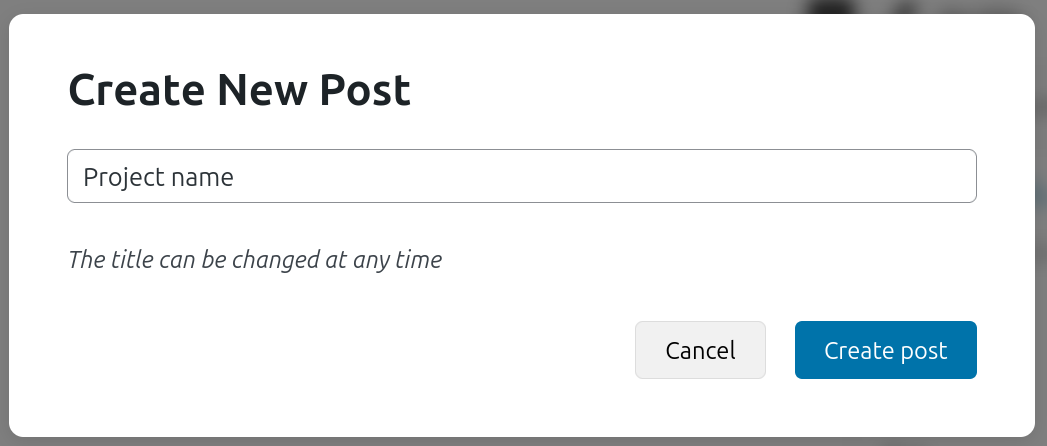
\includegraphics[width=.7\linewidth]{Image/Process/Name.png}
        \caption{Give it a Name}
        \label{fig:name}
    \end{subfigure}
    \bigskip
    %\vspace{.1cm}
    \begin{subfigure}[b]{\textwidth}
        \centering
        
\includegraphics[width=.7\linewidth]{Image/Process/upload.png}
        \caption{Final render}
        \label{fig:first_upload}
    \end{subfigure}
    \caption{Create the post}
\end{figure}

\newpage
\subsection*{Update the settings of the Post}\label{ssec:settings}
\begin{enumerate}
    \item Open the [Settings of the Post] > Click [Post] > Upload the image using [Set featured image] (Fig \ref{fig:featured_image})
    \item Copy the Abstract
    \item Click [Add an excerpt...] > Paste the Abstract (Fig \ref{fig:excerpt})
    \item Click on the Slug > Change it to project-{ID} with the ID of the project (Fig \ref{fig:slug})
    \item The settings should then look like Figure \ref{fig:final_settings}
\end{enumerate}
\

\begin{figure}[h!]
    \centering
    \begin{subfigure}[b]{0.4\textwidth}
        \centering
        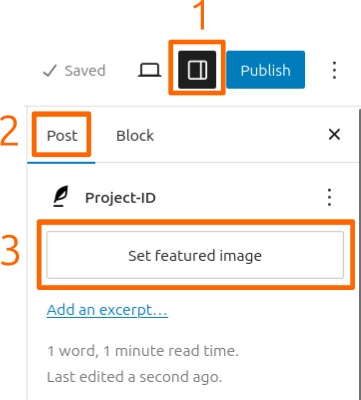
\includegraphics[width=\textwidth]{Image/Process/featured_image.png}
        \caption{Set featured image}
        \label{fig:featured_image}
    \end{subfigure}
    \hfill
    \begin{subfigure}[b]{0.4\textwidth}
        \centering
        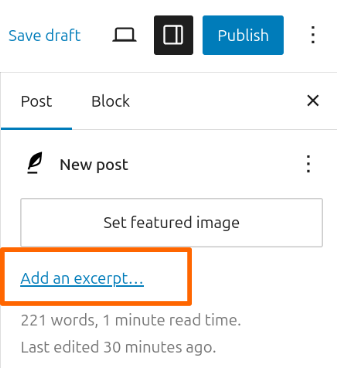
\includegraphics[width=\linewidth]{Image/Process/excerpt.png}
        \caption{Change excerpt}
        \label{fig:excerpt}
    \end{subfigure}
    \bigskip
    \vspace{.1cm}
    \begin{subfigure}[b]{0.6\textwidth}
        \centering
        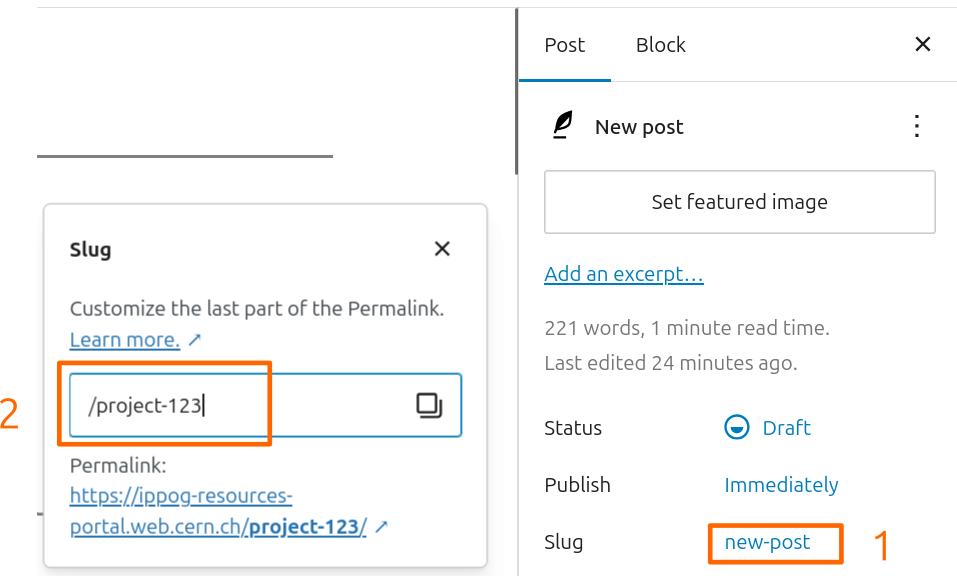
\includegraphics[width=\textwidth]{Image/Process/slug.png}
        \caption{Change the slug}
        \label{fig:slug}
    \end{subfigure}
    \hfill
    \begin{subfigure}[b]{0.3\textwidth}
        \centering
        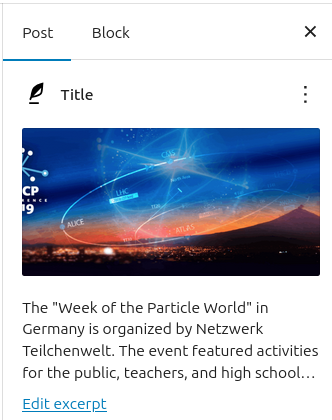
\includegraphics[width=\linewidth]{Image/Process/final_settings.png}
        \caption{Final settings render}
        \label{fig:final_settings}
    \end{subfigure}
    \caption{Settings}
\end{figure}

\newpage
\subsection*{Format the title field}\label{ssec:title}
\begin{enumerate}
    \item Create a block \gray{/media \& text} 
    \item Select [Use featured image] > [Show media on the right] (\ref{fig:media_text})
    \item Create a block \gray{/Title} on the left text field and choose [H1 size]
    \item (optional) Write the subtitle in [H2 size] if there is one
    \item Put the Credit text [aligned right]
    \item Remove all the text beginning with [draft] (\ref{fig:title_final})
\end{enumerate}
\

\begin{figure}[h]
    \centering
    \begin{subfigure}[b]{\textwidth}
        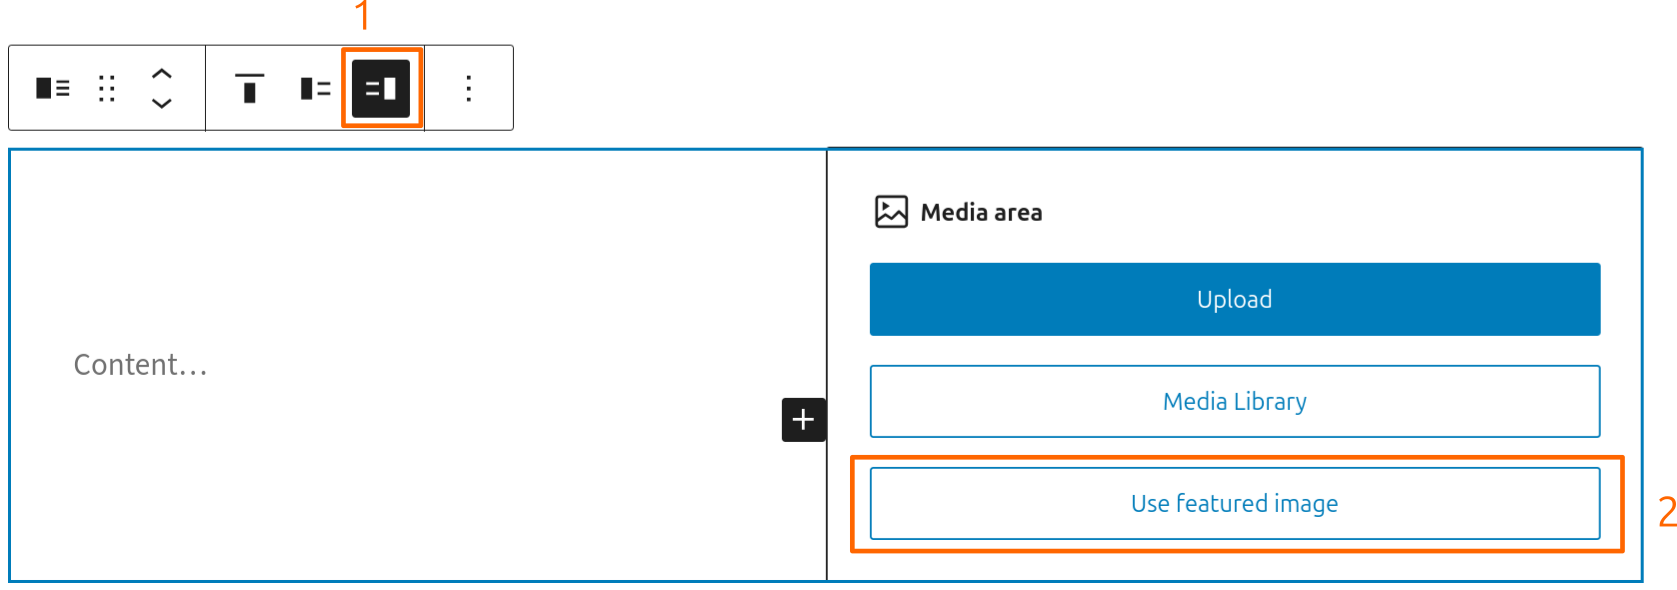
\includegraphics[width=\linewidth]{Image/Process/media_text.png}
        \caption{Media \& Text block}
        \label{fig:media_text}
    \end{subfigure}
    \bigskip
    \vspace{.1cm}
    \begin{subfigure}[b]{\textwidth}
        \centering
        
\includegraphics[width=\linewidth]{Image/Process/title_final.png}
        \caption{Final rendering of the title field}
        \label{fig:title_final}
    \end{subfigure}
    \caption{Title field}
\end{figure}

\newpage
\subsection*{Complete the categories and tags field}\label{ssec:categories}
\begin{enumerate}
    \item Create blocks \gray{/categories} and \gray{/tags}
    \item Respectively add "Categories: " and "Tags: " as prefixes (Fig \ref{fig:tags_categories})
    \item Open the [Settings of the Post] > Click [Post] > Remove "Miscellaneous" and complete the missing tags and categories (Fig \ref{fig:tags_categories_settings})
    \item Remove all the text beginning with [draft]
    \item Change the length of Separators to wide
    \item Finally, publish the article as it is (Fig \ref{fig:publish})
\end{enumerate}

\begin{figure}[th]
    \begin{subfigure}[c]{.5\textwidth}
        \centering
        \begin{subfigure}[t]{\textwidth}
            \centering
            
\includegraphics[width=.7\textwidth]{Image/Process/tags_categories.png}
            \caption{Tags and Categories display}
            \label{fig:tags_categories}
        \end{subfigure}
        
             
        \vspace{5cm}
        \begin{subfigure}[b]{\textwidth}
            \centering
            
\includegraphics[width=.7\textwidth]{Image/Process/publish.png}
            \caption{Publish the Post}
            \label{fig:publish}
        \end{subfigure}
    \end{subfigure}
        \hfill  % NOTE1: hfill moves horizontally stacked objects as far apart as it can
    \begin{subfigure}[c]{.4\textwidth}
        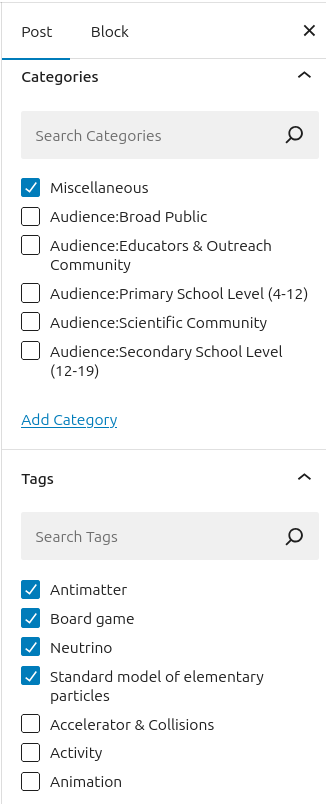
\includegraphics[width=\textwidth]{Image/Process/tags_categories_settings.png}
        \caption{Tags and Categories settings}
        \label{fig:tags_categories_settings}
    \end{subfigure}
    \caption{Uploading the projects}
\end{figure}